The quality control and quality assurance procedures for the individual components of the ProtoDUNE-SP detector are collected in this chapter.

%%%%%%%%%%%%%%%%%%%%%%%%
\section{APA}

%%%%%%%%%%%%%%%%%%%%%%%%
\subsection{General}

Each ProtoDUNE-SP APA will be subject to a testing program during production that will demonstrate their compliance with the design and manufacturing requirements for the experiment.  Given the large size of the APAs, and the highly specialized cryogenic and electronic infrastructure necessary for their designed operation, the testing plan followed during production is necessarily targeted at those features of the APAs which can be addressed prior to final installation in the cryostat.  A separate suite of testing, in a cryogenic environment, is planned to be conducted at CERN, as described in ???? \fixme{is there a section in the TDR for this cold-box test?}.

The tests described in this section will be conducted on APAs during construction, as well as on completed APAs.  Subcomponents ($e.g.$ - wire boards, BeCu wire, etc..) are verified or tested by the appropriate vendor or subsystem manager prior to their use in APA construction.  Each APA will be subject to the testing listed in Table \ref{tab:apatesting}.   Many of the tests (e.g. - tension, continuity, isolation, position survey, bias voltage) are repeated as each successive wire layer of the APA is added, testing the newly installed wires as well as spot-checking wires from previously installed layers. The summary of the tests on each APA, and the associated data collecting during the tests, are recorded in a traveler.

\begin{cdrtable}[APA Testing]{llr}{apatesting}{Tests to be conducted on APAs during production.}
Label & Requirement & Test Method  \\ \toprowrule
Tension      & All wires must be tensioned to 5$\pm$1 N & Laser Survey \\ \colhline
Cryo       &  All APA must operate at 87 K  & Cryotest \\ \colhline
Electrical       & All wires electrically connected at top/bottom of APA  & Continuity \\ \colhline
Isolation & Neighboring APA wires have $\geq$1 M$\Omega$ resistance & Multimeter\\ \colhline
Voltage & Anode planes must hold $\geq$100$\%$ bias & Bias \\ \colhline
Position & All wires must be within 500 $\mu$m of design location & Survey\\ \colhline
Frame & APA frame satisfies all bow/twist/fold criteria & Survey\\ \colhline
\end{cdrtable}

 %%%%%%%%%%%%%%%%%%%%%%%%
\subsection{Tests and surveys}

\fixme{Moved from chap 2}

 %%%%%%%%%%%%
 \subsubsection{Tension survey}

Wire tension is a critical parameter in the performance of the APA, and needs to be strictly controlled to ensure the detector will be robust to operation in a cryogenic environment.  As each wireplane layer is added to the APA, and before the next layer is added and restricts access, the tension of every newly added wire will be measured.  Any wire that is more than 1.0 N out of tolerance from the design value of 5.0 N will be removed and, if possible, replaced.  The tension measurement is performed using a laser-photodiode system, developed at PSL and integrated into the wire-winding apparatus, which will record the resonant frequency of a plucked wire.  Visible checks will also be made during production to identify any noticeably sagging wires.  Spot checks of tension will also be made after cryogenic testing at the production site, as well as at CERN prior to insertion of an APA into the ProtoDUNE-SP cryostat.  

 %%%%%%%%%%%%
\subsubsection{Electrical continuity test}

The electrical connection of each APA wire to the cold readout electronics must be verified to ensure a minimum ($<$0.5$\%$) of un-reachable channels in the completed detector.  Un-reachable wires (e.g. originating from cold solder joints or wires that are broken but held in place by epoxy bead) are distinct from clearly broken wires (e.g. obvious strands of wires hanging loose from the APA) which will be removed/replaced during production.   In addition to providing a pathway to record detector signals, wires receive their bias voltage via their connection to the readout electronics, which shapes the electric field in the anode region.  As such, disconnected wires impact the signals that surrounding channels will collect.  As each wireplane layer is added to the APA, and before the next layer is added and restricts access, the electrical connection of every newly added wire to the corresponding wire-bonding board will be verified.  Using a multimeter, or other equivalent methods, the continuity will be verified by directly probing between the ``bottom" end (i.e. - the end that terminates on the non electronics-plate end of the APA) of the wire and the signal trace on the wire-bonding board at the ``top" end (i.e. - the end that terminates on the electronic-plate end of the APA).  Any wire that fails this continuity test, by producing a resistance $>$ 500 $\Omega$ (using 4.4 $\Omega$/m resistance for BeCu wire that is 7.5 m long, and allowing margin for additional parasitic resistance), will be removed and, if possible, replaced.  Spot checks of continuity will also be made after cryogenic testing at the production site, as well as at CERN prior to insertion of an APA into the ProtoDUNE-SP cryostat.

 %%%%%%%%%%%%
\subsubsection{Electrical isolation test}

Each wire of the APA should be electrically isolated from every other wire, in order to avoid shorting out channels and potentially damaging the readout electronics.  Shorted-out wires will also impact the electric-field uniformity in the anode region, and can impact signals in surrounding channels.  Using a multimeter, or other equivalent methods, the isolation between each APA wire and adjacent wires will be measured and verified to have resistance $>$ 1 M$\Omega$.  Since a given wire has many adjacent wires, a dedicated circuit designed to expedite this test will be desirable.  Any wire failing this test will be removed and, if possible, replaced.  Visible checks will also be made during production to identify any touching wires.  Spot checks of isolation will also be made after cryogenic testing at the production site, as well as at CERN prior to insertion of an APA into the ProtoDUNE-SP cryostat.

 %%%%%%%%%%%%
\subsubsection{Wire position survey}

Knowledge of the position of every wire in the APA is required in order for physics analysis of data to be successful.  This information is utilized to create a description of the detector geometry inside the simulation software, and is the basis on which reconstruction algorithms are built. The preliminary description of the geometry assumes a perfect detector built according to the APA design drawings.  Any deviations from this design in the final as-built APAs needs to be incorporated into the software geometry.  All wires should be surveyed during production to verify they are within 500 $\mu$m of the design location.  This survey is partially accomplished by verifying the APA flame flatness is within specifications, and that the wire-bonding boards and support combs are located upon the frame in the desired position.  The APA will be surveyed using a Cognex camera integrated into the winding machine.  The camera employs machine vision to identify each pin/tooth on the installed wire-bonding boards, and from this data a map of wire location will be generated.  This survey should be performed as each wireplane layer is added to the APA, and before the next layer is added and restricts access.  Any wire that is more than 500 $\mu$m from the nominal location, according to survey data, should be inspected and if found to have problems, removed and replaced.  Visual checks throughout the wire-winding process will also be performed to identify any wires that appear out of place.

 %%%%%%%%%%%%
\subsubsection{Bias voltage test}

All wires on the APA must be able to reach their design bias voltage in order to achieve the desired electric-field uniformity and transparency conditions required for successful LArTPC operation.  Inability to reach the desired voltage could be an indication of component failure on the CR boards, or of wires in the APA being shorted out.  The CR boards should be tested prior to their installation on the APA to verify they can be biased to 100$\%$ of the largest operating voltage of any anode layer (e.g. the Collection layer's 820 V).  The components selected for the CR boards are chosen with margin about this operating point, to allow for bias voltages in the as-built detector to be adjusted, either for signal-shaping studies or for systematic studies of detector performance at various drift-field values.  As each wireplane layer is added to the APA, and before the next layer is added and restricts access, each newly added wire-bonding board should be connected to a CR board and biased to 100$\%$ of the largest operating voltage of any anode layer.  Any unexpected current draws observed will be traced to the originating wire(s), and if necessary, the offending wire(s) will be replaced.  Visual checks should also be performed during this test to verify that wires being biased do not deflect or move in any unexpected manner.  This test may be augmented when multiple wireplane layers are available, to verify that wires in adjacent layers do not develop unexpected cross-talk when biased.

 %%%%%%%%%%%%
\subsubsection{Cryogenic test}

The completed APAs must be robust to operation in a cryogenic environment.  Wires must be able to withstand the cooldown to liquid argon temperatures.  In order to verify the workmanship of each APA, a cryogenic test will be performed as each APA is completed and before shipment to CERN.  The APAs will be placed in a custom-built cold box, where they will be gradually cooled (at a rate consistent with requirements on keeping wire tension increases below a safe level) to $\sim$100 K (exact value to be determined).  The default plan is to use cold gas from a LN supply for this test, and flush gas through the cold box until it reaches the desired temperature.  The APA will be arranged in a horizontal orientation, as this simplifies the engineering of the cold box.  It is not anticipated that loading on the APA/wires due to gravity (e.g. from horizontal vs. vertical orientation) will lead to any significant changes in wire tension, and the frame will be supported appropriately.  The APA will be inspected after this cold test to verify that no wires have broken.  Spot-check tests of tension/continuity/isolation/bias will be performed to verify if any channels have changed relative to their pre cold-test values.  Criteria for acceptance after this test (e.g. number of problematic wires identified by this test) are under development.

 %%%%%%%%%%%%
\subsubsection{Testing at CERN}

Upon arrival at CERN, and prior to integration with interfacing subsystems (e.g. - light collection and electronics), each APA will be subjected to visual inspection, and spot-check ($\sim$10$\%$ of total channels) tests for wire tension, continuity, isolation, and bias voltage will be performed and compared to the equivalent pre-shipping values.




%%%%%%%%%%%%%%%%%%%%%%%%
\section{CPA}

The following activities are planned to assure the CPA meets all design requirements as defined in the fabrication drawings and description in the sections above:
\begin{itemize}
\item Performed 35 ton HV test at FNAL.
\item Fabricate four prototype CPAs to test the design and fabrication and assembly methods.
\item Installation test at Ash River:
\begin{itemize}
\item Test the lifting and handling of the four prototype CPA's.
\item  Load the 4 prototype CPA's with FC modules and test and evaluate their installation.
\end{itemize}
\item Develop a QC plan for inspecting every fabricated part of the CPA frame to make sure they meet the dimensions and tolerances on the fabrication drawings.
\item Develop a QC plan for inspecting and measuring each CPA module and completed CPA plane to ensure they meet the dimensions and tolerances on the drawings.
\item Perform tests of each joint in the CPA frame (see Section 3) to ensure that their design and strength meets the load requirements.
\item Create an integrated model of the entire TPC to evaluate interfaces and installation methods.  
\item Develop a QC for receiving the resistive panels.  Measure the dimensions to confirm they meet the drawings and setup a plan and acceptance criteria to insure that panel resistance is acceptable.
\item Develop a QC  HV test at CERN for evaluating side to side and top to bottom resistance for each completed CPA but after final assembly and after hanging during installation.  
\end{itemize}

%%%%%%%%%%%%%%%%%%%%%%%%%
\section{FC}

The following activities are/will be performed to assure the field cage meets all design criteria as defined in the fabrication drawings and description in the sections above:
\begin{itemize}
\item	Fabricate prototype FCs to test the design and fabrication and assembly methods.
\item	Installation test at Ash River:
\begin{itemize}
\item	Test the lifting and handling of the prototype FCs.
\item	Mount the prototype FCs to the CPA modules and test and evaluate their installation.
\end{itemize}
\item	Develop a QC plan for inspecting every fabricated part of the FC frame to make sure they meet the dimensions and tolerances on the fabrication drawings.
\item	Develop a QC plan for inspecting and measuring each FC module and completed FC plane to insure they meet the dimensions and tolerances on the drawings.
\item	Perform tests of each joint in the FC frame (see Section XX) to insure that their design and strength meets the load requirements.
\item	Create an integrated model of the entire TPC to evaluate interfaces and installation methods.  
\end{itemize}

 %%%%%%%%%%%%%%%%%%%%%%%%%
\section{HV}

\fixme{no info contributed}

  %%%%%%%%%%%%%%%%%%%%%%%%%
\section{PDS}

\fixme{no info contributed}

%%%%%%%%%%%%%%%%%%%%%%%%%
\section{CE}

A full description of the testing procedures is being developed in a separate document. A 
summary is provided here.

%%%%%%%%%%%%%%%%%%%%%%%%%
\section{DAQ}

The DAQ for ProtoDUNE-SP does not require large numbers of custom hardware components to 
be built and tested.  There will be 8 COBs with 8 RCEs each, 2 FELIX cards, 24 SSPs, the timing 
and trigger systems and off-the-shelf hardware (computers, network switches, storage, etc.).
As such, a significant amount of automation is not needed to test and qualify the 
components.  

Qualification tests of the RCEs, FELIX boards, SSPs, timing and trigger systems will
be driven by the host institutes producing those systems.  Reception tests will be 
performed to identify any failures due to transport.  In order to fully qualify the 
boards, they will need to be individually tested with control samples.  Data generators
will be used in place of the front-end electronics where applicable.  Full data rate 
testing will be performed when the first full detector slice is in place at EHN1 (expected
Q2 2017).  Data challenges will take place during Q1 2017 in advance of the arrival of the 
first APA, and again as the computing system expands to its full capacity.

%%%%%%%%%%%%%%%%
\subsection{Prototype testing}
\label{subsubsec:ce_install_proto}

Dedicated test boards for the FE ASIC and ADC ASIC,
were used to characterize the performance of prototype ASICs at both 300~K and 77~K,
and taking them through multiple thermal cycles.
An automated test board was built for the FE ASIC (Fig.~\ref{fig:tpcce_FE_TestBoard})
to evaluate large numbers of FE ASICs at room temperature,
and another such board is currently being designed for the ADC ASIC (Fig.~\ref{fig:tpcce_ADC_TestBoard}).

\begin{cdrfigure}[FE ASIC testboard]{tpcce_FE_TestBoard}{FE ASIC testboard.}
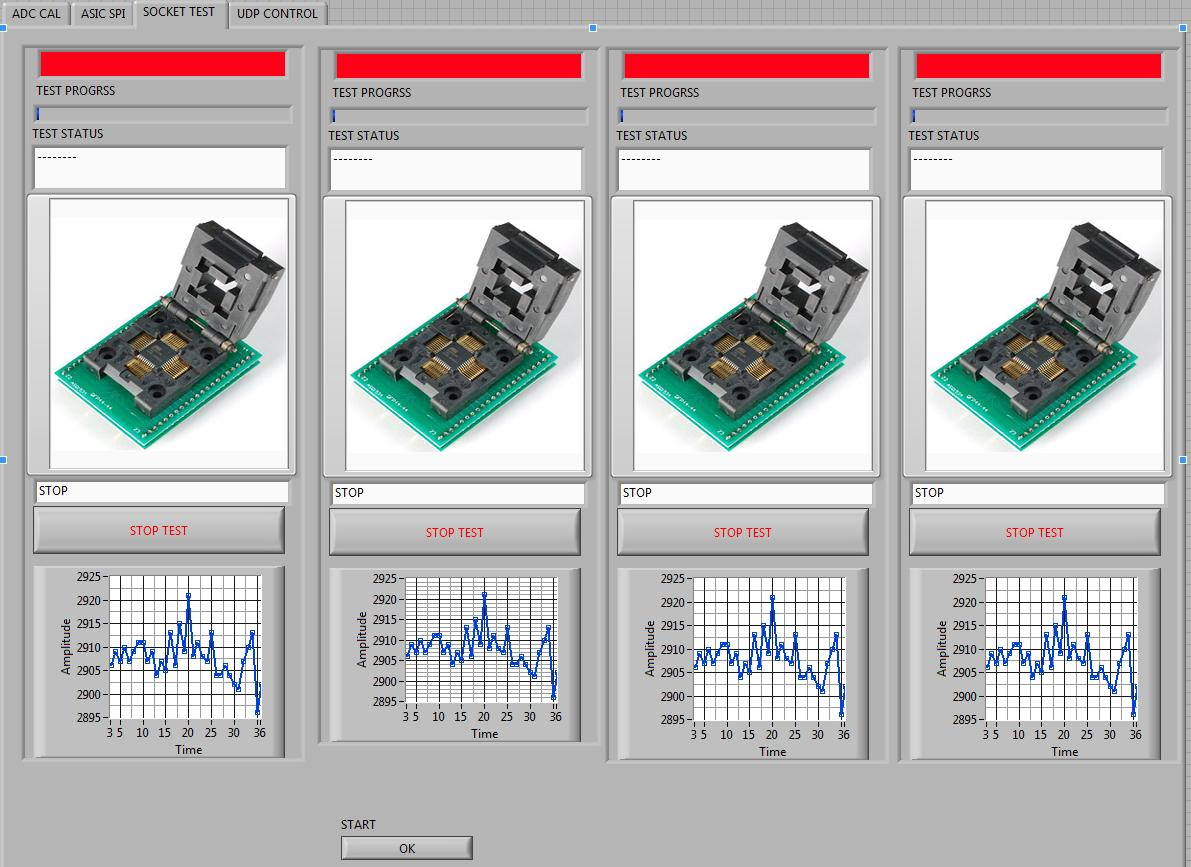
\includegraphics[width=0.6\linewidth]{tpcce_FE_TestBoard}
\end{cdrfigure}
\begin{cdrfigure}[ADC ASIC testboard]{tpcce_ADC_TestBoard}{ADC ASIC testboard.}
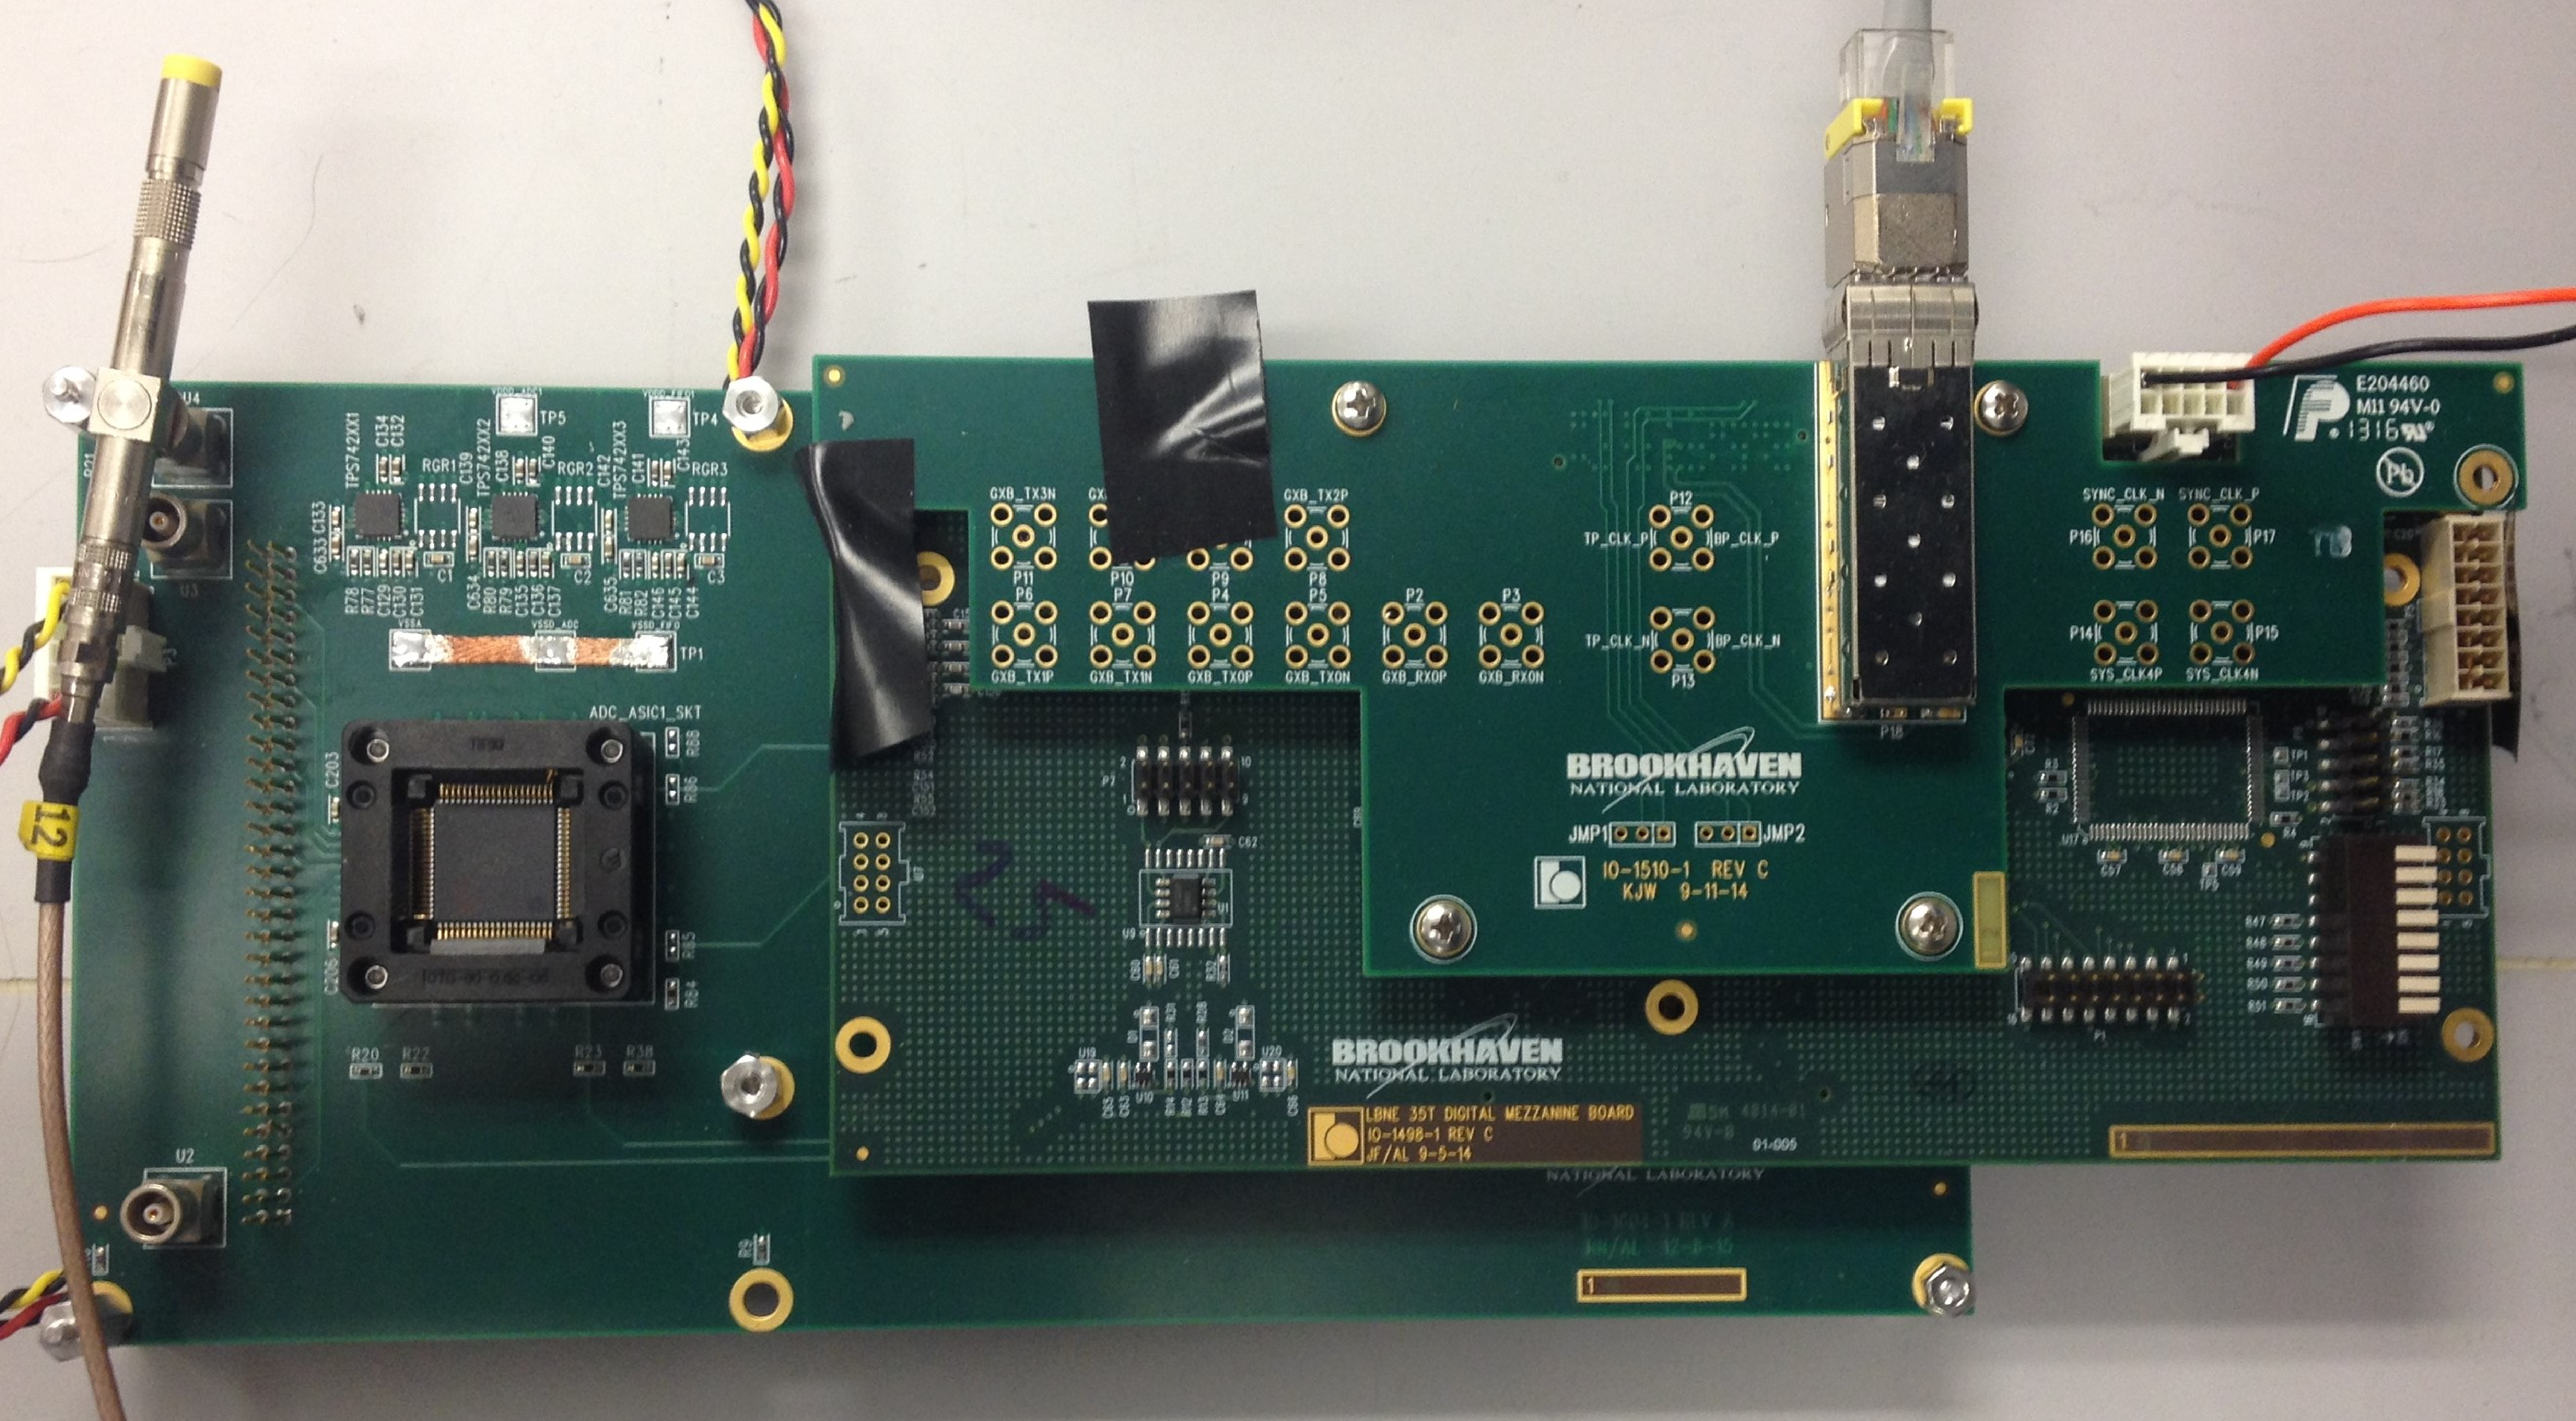
\includegraphics[width=0.6\linewidth]{tpcce_ADC_TestBoard}
\end{cdrfigure}

The development of the FE and ADC ASICs has proceeded through a series of prototype designs.
A 128-channel prototype analog mother board has been developed and tested in the lab.
Together with an FPGA mezzanine in place of the digital ASIC mezzanine,
they form a FEMB for use in the protoDUNE TPC,
since the COLDATA work is unlikely to be advanced enough to
provide more than a fraction of the electronics needed for the aggressive protoDUNE schedule.
A test stand has been developed to test the FEMB
using a commercial FPGA evaluation board as a mini-DAQ system.
All evaluation test data are stored on a desktop PC and analyzed to
determine whether the board is ready to be installed on the detector.

During the prototype testing, a procedure has been developed for the production test of the cold electronics boards.
This includes key parameters (gain, noise, non-linearity, etc.) that should be tested,
detailed steps of the test to collect data and extract these parameters,
and also the work flows to perform the test at both 300~K and 77~K.

Prototype cold electronics has been tested with prototype TPC and DAQ system,
to evaluate the performance of the APA assembly, and help the development of the DAQ software.
A vertical slice test has been used as the test bed for the integration test.
It is an important step to identify potential issues, check out system integration and performance
before the installation into the cryostat.

%%%%%%%%%%%%%%%%
\subsection{CE assembly testing}
\label{subsubsec:ce_install_assembly}

The front-end readout boards will be thoroughly tested. A testing program has been identified:
\begin{itemize}
\item A small number of the ASICs will undergo a complete suite 
of tests, including thermal cycling to determine the batch yield.
\item If the yield is high ($>$ 95\%), all ASICs will be mounted 
on the front-end boards.
Tests will be performed on each board and bad chips replaced as needed.
\item If the yield is not high, an automated test fixture will be 
fabricated to validate every ASIC chip before mounting on the readout boards.
Board-level tests after mounting the ASICs will be conducted.
However, previous experience indicates that this scenario is very unlikely.
\item The fully assembled front-end boards will be thermally cycled multiple times while connected
to a simple DAQ system to ensure reliable operation.
\item After the front-end electronics boards have been installed on an APA,
an initial calibration of all electronic channels will be performed.
The electronic gains and noise levels of all channels will be recorded in a database.
\item Electronic calibration on all channels will be performed while the APA is cold and again after it is warmed up.
\end{itemize}

%%%%%%%%%%%%%%%%%%%%%%%%%
\section{Beam plug}

As a part of the QC process for the beam plug, the vendor will conduct the following acceptance tests for the production units before shipping:
\begin{itemize}
\item {Initial helium leak check}
\item {Internal pressure check at cryogenic temperature (at about 2x operating pressure)}
\item {Post-test helium leak check to assess potential damage}
\item {External pressure check at room temperature (below 100 psi)}
\item {Final helium leak check to ensure no damage has been incurred}
\end{itemize}
The acceptable leak rate is below 15.6$\times 10^{-5}$ scc/s (He gas equivalent).
The tests performed by the vendor are primarily related to pressure safety and leak rates. Some of those tests will be repeated by LBNL upon receiving the units to verify vendor's results. In addition, LBNL will conduct tests to verify other aspects of the beam plug, in particular, the HV characteristics. The HV tests will be conducted using various facilities as described in the following sections.

\paragraph{BLANCHE Test Stand}
The BLANCHE test stand at Fermilab is a LAr cryostat dedicated to study high voltage related issues. It is 152 cm tall with a 76 cm inner diameter. The test stand is connected to a LAr purification system to remove oxygen and water contamination. The test stand is capable of delivering up to 150 kV to the sample. The cryostat is large enough to test a full size beam plug. The plan is to test the beam plug in BLANCHE to verify that the beam plug can withstand HV in LAr environment.
\\fixme{earlier nominal value across beam plug was said to be 165kV - so, test is not covering full range. Maybe add sentence to address this issue.}

\paragraph{Test in Charged Particle Beam}
During ProtoDUNE-SP physics runs, a charged particle beam will go through the beam plug with a rate of up to 100 Hz during a beam spill. The current induced from the ionization of the nitrogen gas by the charged beam particles is expected to be small; less than 1 nA during the spill. Given the low ionization rate and long pause between spills, we do not expect the charged particle beam to introduce electrical breakdown inside the beam plug. However, we plan to verify the design by putting the beam plug in a test beam with the beam plug at nominal HV. We will study the current flow inside the beam plug as a function of beam rate and nitrogen gas pressure. To minimize possible HV breakdown on the outer surface of the beam plug, which may complicate the interpretation of the test results, the beam plug will be immersed in dielectric oil. The test apparatus with the beam plug installed inside the setup is shown in Figure~\ref{fig:beamwindow_SLAC}.
\begin{cdrfigure}[SLAC beam test]{beamwindow_SLAC}{Beamplug test setup in electron beam to test electrical breakdown in the N filler gas.}
  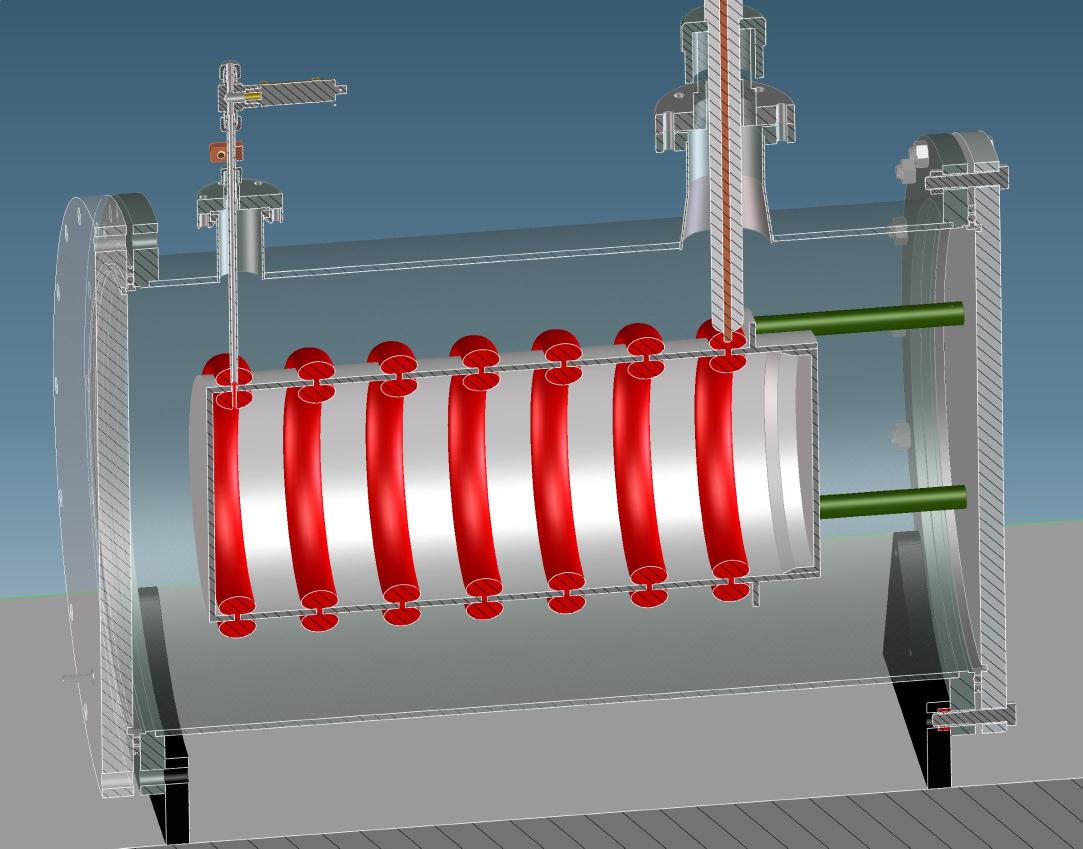
\includegraphics[width=0.6\textwidth]{beamwindow_SLACtest}
\end{cdrfigure}

\paragraph{Full integration test in 35-ton cryostat}
The final QC test of the beam plug is conducted inside the 35-ton cryostat at Fermilab. A small field cage mock-up is constructed and assembled inside the cryostat along with the beam plug. For this test, the beam plug is mounted to the field cage using a mounting scheme which is identical to the ProtoDUNE-SP one. The field cage mock-up will only have the first 10 profiles of a TPC, however, they will be operating at the nominal voltages. Therefore, the planned test will be a full-field test with the beam plug integrated into the field cage and the rest of the HV systems. A successful test would entail operating the TPC at the nominal HV (CPA at -180 kV) with the beam plug attached and that the electrical performance of the field cage with and without the beam plug is functionally the same.

\begin{cdrfigure}[PC4 Test setup]{beamwindow_PC4}{Field cage mock-up high voltage test in 35-ton cryostat \fixme{preliminary drawing}.}
  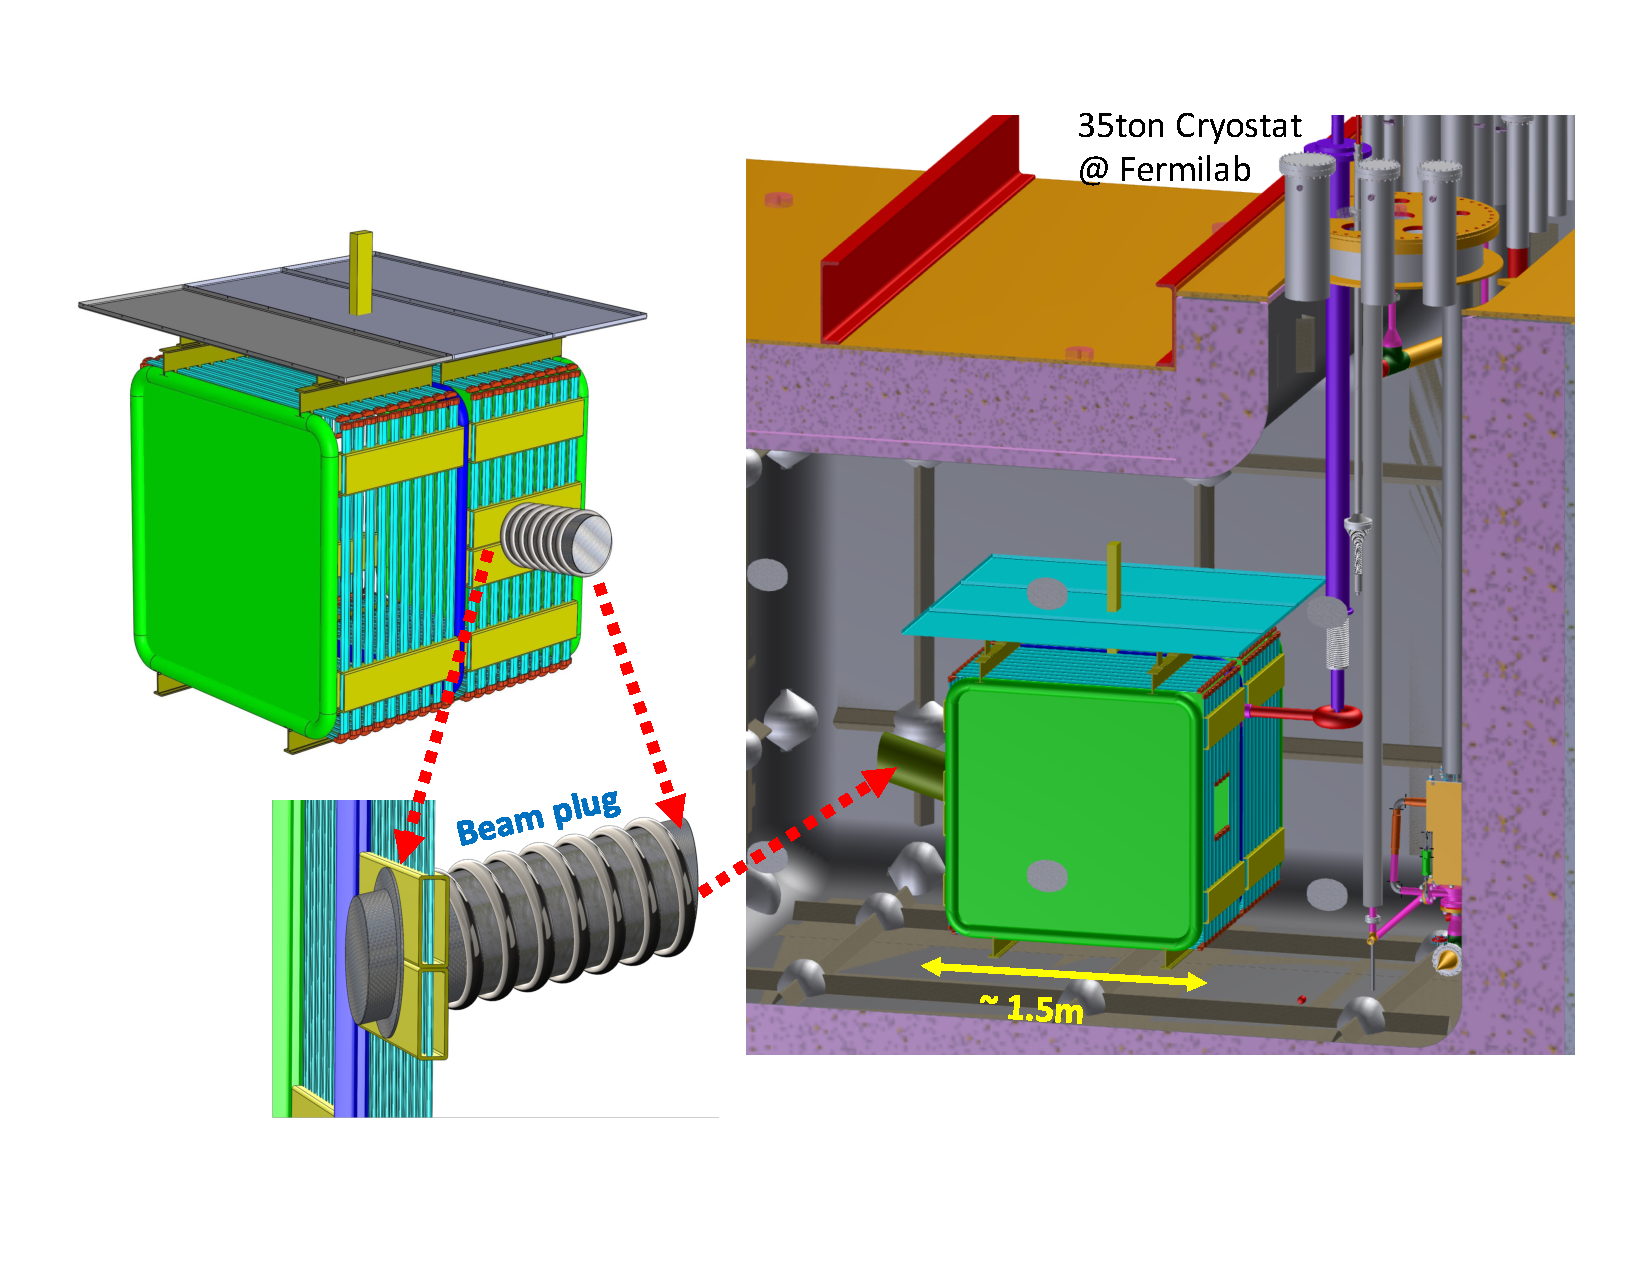
\includegraphics[width=0.95\textwidth]{beamwindow_PC4Test}
\end{cdrfigure}

%%%%%%%%%%%%%%%%%%%%%%%%%
\section{Cryogenics and LAr purification systems}

%%%%%%%%%%%%%%%%%%%%%%%%%
\subsection{Scope}

The project follows the CERN QA/QC plan. Additionally, specific Neutrino Platform Cryogenics documentation control policies have been developed to ensure that the documentation is circulated and archived properly. A design plan is also being developed to ensure that the design is performed according to the specifications.\\
%
External companies will be contracted for the design, fabrication, delivery, installation and testing of the cryogenic system, one for the proximity and external cryogenics and one (could be the same) for the internal cryogenics.

The following sections are extracts from the \textit{Quality Assurance} section of the Invitation to Tender for the proximity and external cryogenics and the Price Enquiry for the internal cryogenics~\cite{invit-tender-cryo}.

%%%%%%%%%%%%%
\paragraph{General}

The contractor shall have or shall guarantee that its sub-contractors (when applicable) have a valid ISO 9001:2008 (or later) certifications issued by a recognized certification body in the scope of the supply for \"design, engineering, production, installation, sales of vacuum systems, cryogenic equipment and transfer lines\".

%%%%%%%%%%%%%
\paragraph{Scope}
A dedicated quality plan must be prepared by the contractor as per requirements.

%%%%%%%
\paragraph{Definition}
A quality plan describes the operational quality system to ensure that:
\begin{itemize}
\item Contract requirements will be met.
\item Evidence of such compliance is maintained.
\end{itemize}
It covers the whole scope of the contract.

%%%%%%%
\paragraph{Content of the quality plan}
\begin{itemize}
\item The specific allocation of resources, duties, responsibilities and authority.
\item Details of all sub-contractors and how interfaces will be managed if any.
\item The specific procedures, methods and work instructions to be applied.
\item The specific procedures for inspection and testing.
\item The specific methods of communication and testing
\item The design and performance margins.
\end{itemize}


%%%%%%%
\paragraph{Quality management}

The plan shall:
\begin{itemize}
\item Identify the key individuals responsible for ensuring the activities performed during the contract.
\item Show an organization flow chart to facilitate understanding.
\end{itemize}

%%%%%%%
\paragraph{Deviations and non-conformities}

The plan shall indicate how, when and by whom deviations and non-conformities will be processed including those originating from subcontractors, if any.

%%%%%%%%%%%%%%%%%%%%%%%%%
\subsection{Cryo and LAr purification inspection and controls}

Specific control points apart from the ones required by the chosen applicable standards and Pressure Equipment Directive (PED) Essential Safety Requirements
 will be performed during the fabrication and installation phases. Every specific inspection or control will be covered by a dedicated procedure developed by the manufacturer and approved by CERN. In case of non-conformities (i.e., non-compliance with specified requirements), a corresponding non-conformity report will be issued by the manufacturer.

The contractor will ensure a close oversight of the manufacturing. This monitoring will include Notification Points (NP) and Hold Points (HP).

A NP is a milestone where the contractor is required to notify CERN that it has completed a specific task or a specific deliverable and is proceeding to the next task or to the next action on the specific deliverable. A NP is meant to enable CERN personnel to follow the progress of the contract and possibly to witness a critical manufacturing step at the contractor' s premises. A NP will not affect the production flow of the contractor that will continue the work even without a reply from CERN. 

A HP is a milestone where contractor is required to notify CERN that it has completed a specific task or a specific deliverable and must stop the associated processes until a HP Clearance is issued. The HP Clearance will be issued on the basis of clearly identified Quality Control, data and acceptance test results to be provided to CERN at the time of the request. In case of clearance, the contractor will resume its activity. In case of rejection, the contractor will develop a recovery plan that will be submitted and reviewed by CERN.

The list of NP and HP to be implemented during the various phases of the execution will be mutually agreed between CERN and the contractor. The minimum inspection and controls that will be performed during fabrication and installation are:

\begin{itemize}
\item Non-destructive test of welds
\item Helium leak tightness test
\item Cold test (during acceptance)
\item Pressure test
\item Cleanliness control
\item Dimensional control
\item Transport acceleration
\item Factory outlet inspection
\item CERN incoming inspection
\item Final position inspection
\item Positioning and layout control
\item Interfaces control
\item Hydraulic continuity control
\item Control of external supports
\end{itemize}


%%%%%%%%%%%%%%%%%%%%%%%%%
\section{Detector monitoring and slow control}

\fixme{missing}

%%%%%%%%%%%%%%%%%%%%%%%%%%%%%%%%%%%%%%%%%%%%%%
%\section{QA/QC and testing space}
\section{Installation space and clean room}
\label{sec:quality:space}

All of the testing for the TPC components will be done inside the clean room or inside the cryostat. 

Once the APAs are moved into the clean room, a connectivity test will be performed to look for shorted or broken wires.  It will also be inspected visually for broken wires.  Tension tests will be performed on some fractions of the wires and the results will be compared to the ones taken at the production facility.

For the PDs, each PD will be unpacked and placed inside a full length dark box with a scanning VUV light source. This will be an identical test set up to the one used at the production facility.  Each test will take approximately 2 hours, which is the planned time for the installation and cabling of a PD into the APA.  

The CE modules will be delivered as an assembly.  The CE enclosure will have the electronics boards mounted inside and the internal cable from the harness connected and tested.  Each module will undergo an acceptance test when they are unpacked inside the clean room.  Once tested, they will be installed on the top of the APA frame from either a scaffold or a scissor lift located in the clean room.  A connectivity test will be performed on each module to ensure the electrical connections.  

After the APA has been fully integrated with the PD and CE, it will be moved via the rails in the clean room to the integrated cold testing stand.  This test stand, shown in Figure \fixme{6}, is a large insulated box that is light tight for PD testing and a Faraday shield for CE testing.  The test stand is shown with an APA inside and the end cover removed.  
%
\begin{cdrfigure}[short caption for table of figures]{label}{6 long caption that appears below picture}
%  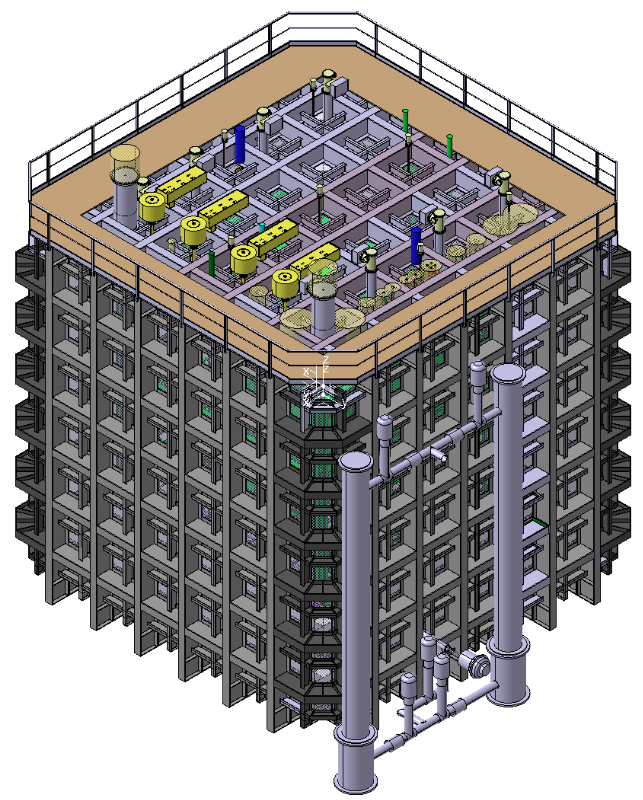
\includegraphics[width=0.8\textwidth]{protoDUNE_cryostat.png}
\end{cdrfigure}
%
At the top of the box, there will be a crossing tube, similar to those in the cryostat, with a conflat fitting that will accept the warm – cold interface flange for the PD and CE cable connections.  The PD and CE cables will be routed and connected to their flanges, the APA will be moved inside and the end cover, that completes the Faraday cage, installed so that the integrated electronics testing can begin.  A series of warm tests will be performed.  This is described in \fixme{need to find... XXsectionXX}.  After the warm tests are complete, the inner volume of the enclosure will be purged with dry gas to reduce the moisture inside.  After this gas purge, the inner volume will be slowly cooled down using nitrogen gas to a temperature of approximately 100 K.  The rate of cooldown is to be less than 10 K/hr which is the same for the cryostat.  The cooldown system is being designed to maintain the inner volume near 100 K for approximately 48 hours.  The cold testing of this can be performed during the cooldown period, during these 48 hr and during the warmup.  After the testing is complete and the box has been purged of nitrogen with room air, it will be opened, the APA removed and the cables disconnected and secured for movement on the rail system.   

Each of the CPA panels will be visually inspected for damage to the resistive coating on the panels.  At the panels are assembled into a CPA module, electrical connections will be made and tested between the panels.  As the modules are mounted on the clean room rails, the modules will be electrically connected between the modules.  This connection will be tested in the clean room and when the CPAs are moved inside the cryostat to their final position.  

The FC assemblies will be visually inspected for damage as they are removed from their shipping containers.  The electrical connections between the divider chains will be tested.  Once attached to the CPA, an electrical connection between the CPA and FC must be made to carry the HV to the FC.  This will be tested in the clean room before moving the assembly into the cryostat. 



